\part{Informatik 1 -- Wintersemester 2008}
\chapter{Physik}
\section{11.12.2008}
\subsection{11.12.2008-IMG-phys-1}
\begin{tikzpicture}
	\draw[thick] (0,0) node [left] {$G$} -- (2,0);
	\draw[thick] (0,0) circle (0.07);
	\draw[thick] (2,1) -- (2,-1);

	\draw[thick] (3,1) -- (3,-1);

	\draw[thick] (3,1) -- (4,1) -- (4,3) node [right] {$D$};
	\draw[thick] (4,3) circle (0.07);

	\draw[thick] (3,-1) -- (4,-1) -- (4,-3) node [right] {$S$};
	\draw[thick] (4,-3) circle (0.07);

	\draw[thick] (3,0) -- (5,0) node [right] {$B$};
	\draw[thick] (5,0) circle (0.07);
\end{tikzpicture}
\begin{lstlisting}[frame=single]
\end{lstlisting}
\begin{tikzpicture}
	\draw[thick] (0,0) node [left] {$G$} -- (2,0);
	\draw[thick] (0,0) circle (0.07);
	\draw[thick] (2,1) -- (2,-1);

	\draw[thick] (3,1) -- (3,-1);

	\draw[thick] (3,1) -- (4,1) -- (4,3) node [right] {$D$};
	\draw[thick] (4,3) circle (0.07);

	\draw[thick] (3,-1) -- (4,-1) -- (4,-3) node [right] {$S$};
	\draw[thick] (4,-3) circle (0.07);

	\draw[thick] (3,0) -- (5,0) node [right] {$B$};
	\draw[thick] (5,0) circle (0.07);
\end{tikzpicture}


\subsection{11.12.2008-IMG-phys-3}
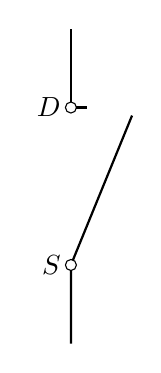
\begin{tikzpicture}
	\draw[thick] (0,0) -- (0,1) node [left] {$S$} -- (75:3);
	\draw[thick] (0.2,3) -- (0,3) node [left] {$D$} -- (0,4);

	\draw[fill=white] (0,1) circle (0.07);
	\draw[fill=white] (0,3) circle (0.07);
\end{tikzpicture}
\begin{lstlisting}[frame=single]
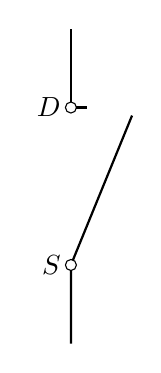
\begin{tikzpicture}
	\draw[thick] (0,0) -- (0,1) node [left] {$S$} -- (75:3);
	\draw[thick] (0.2,3) -- (0,3) node [left] {$D$} -- (0,4);

	\draw[fill=white] (0,1) circle (0.07);
	\draw[fill=white] (0,3) circle (0.07);
\end{tikzpicture}
\end{lstlisting}

\subsection{11.12.2008-IMG-phys-4}
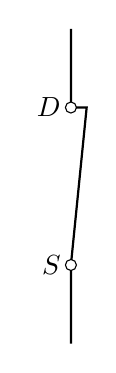
\begin{tikzpicture}
	\draw[thick] (0,0) -- (0,1) node [left] {$S$} -- (0.2,3) -- (0,3) node [left] {$D$} -- (0,4);

	\draw[fill=white] (0,1) circle (0.07);
	\draw[fill=white] (0,3) circle (0.07);
\end{tikzpicture}
\begin{lstlisting}[frame=single]
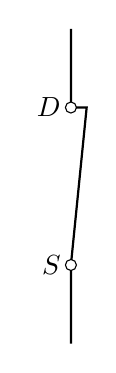
\begin{tikzpicture}
	\draw[thick] (0,0) -- (0,1) node [left] {$S$} -- (0.2,3) -- (0,3) node [left] {$D$} -- (0,4);

	\draw[fill=white] (0,1) circle (0.07);
	\draw[fill=white] (0,3) circle (0.07);
\end{tikzpicture}
\end{lstlisting}

\subsection{11.12.2008-IMG-phys-6}
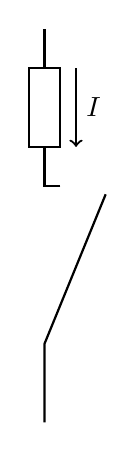
\begin{tikzpicture}
	\draw[thick] (0,0) -- (0,1) -- (75:3);
	\draw[thick] (0.2,3) -- (0,3) -- (0,5);

	\draw[thick, fill=white] (-0.2,3.5) rectangle (0.2,4.5);

	\draw[->, thick] (0.4,4.5) -- (0.4,3.5) node [midway, right] {$I$};
\end{tikzpicture}
\begin{lstlisting}[frame=single]
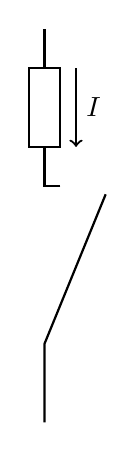
\begin{tikzpicture}
	\draw[thick] (0,0) -- (0,1) -- (75:3);
	\draw[thick] (0.2,3) -- (0,3) -- (0,5);

	\draw[thick, fill=white] (-0.2,3.5) rectangle (0.2,4.5);

	\draw[->, thick] (0.4,4.5) -- (0.4,3.5) node [midway, right] {$I$};
\end{tikzpicture}
\end{lstlisting}

\subsection{11.12.2008-IMG-phys-7}
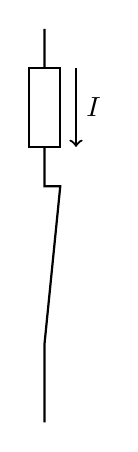
\begin{tikzpicture}
	\draw[thick] (0,0) -- (0,1) -- (0.2,3) -- (0,3) -- (0,5);

	\draw[thick, fill=white] (-0.2,3.5) rectangle (0.2,4.5);

	\draw[->, thick] (0.4,4.5) -- (0.4,3.5) node [midway, right] {$I$};
\end{tikzpicture}
\begin{lstlisting}[frame=single]
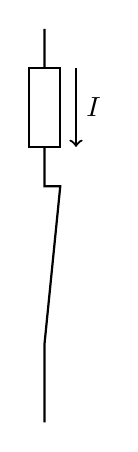
\begin{tikzpicture}
	\draw[thick] (0,0) -- (0,1) -- (0.2,3) -- (0,3) -- (0,5);

	\draw[thick, fill=white] (-0.2,3.5) rectangle (0.2,4.5);

	\draw[->, thick] (0.4,4.5) -- (0.4,3.5) node [midway, right] {$I$};
\end{tikzpicture}
\end{lstlisting}

\section{22.12.2008}
\subsection{22.12.2008-IMG-phys-1}
\begin{tikzpicture}
	\draw[thick, ->] (0,-0.5) -- (0,6) node[left] {$z$};
	\draw[thick, ->] (-0.5,0) -- (8,0) node[below] {$x$};
	\draw[thick, ->] (-0.25,-0.25) -- (4,4) node[right] {$y$};

	\draw[draw=green, ->] (0,0) -- (4.5,-0.5);
	\draw[draw=blue, ->] (0,0) -- (2.5,1.5);
	\draw[draw=red, ->] (0,0) -- (0.5,3);

	\fill[green] (0,0) circle (3pt);
\end{tikzpicture}
\begin{lstlisting}[frame=single]
\begin{tikzpicture}
	\draw[thick, ->] (0,-0.5) -- (0,6) node[left] {$z$};
	\draw[thick, ->] (-0.5,0) -- (8,0) node[below] {$x$};
	\draw[thick, ->] (-0.25,-0.25) -- (4,4) node[right] {$y$};

	\draw[draw=green, ->] (0,0) -- (4.5,-0.5);
	\draw[draw=blue, ->] (0,0) -- (2.5,1.5);
	\draw[draw=red, ->] (0,0) -- (0.5,3);

	\fill[green] (0,0) circle (3pt);
\end{tikzpicture}
\end{lstlisting}

\subsection{22.12.2008-IMG-phys-2}
\begin{tikzpicture}
	\draw[thick, draw=blue, ->] (0,0) -- (0,-7);
	\draw[thick, draw=blue, ->] (2,0) -- (2,-7);
	\draw[thick, draw=blue, ->] (4,0) -- (4,-7);
\end{tikzpicture}
\begin{lstlisting}[frame=single]
\begin{tikzpicture}
	\draw[thick, draw=blue, ->] (0,0) -- (0,-7);
	\draw[thick, draw=blue, ->] (2,0) -- (2,-7);
	\draw[thick, draw=blue, ->] (4,0) -- (4,-7);
\end{tikzpicture}
\end{lstlisting}

\subsection{22.12.2008-IMG-phys-5}
\begin{tikzpicture}
	\draw[thick, dashed, draw=blue] (0,0) rectangle (9,7);
	\draw[thick, draw=blue] (1,1) node[text=blue] {$\times$} circle (0.25);
	\draw[thick, draw=blue] (8,1) node[text=blue] {$\times$} circle (0.25);
	\draw[thick, draw=blue] (1,6) node[text=blue] {$\times$} circle (0.25);
	\draw[thick, draw=blue] (8,6) node[text=blue] {$\times$} circle (0.25);
	\node[text=blue, above] at (4.5,7) {\LARGE{$\vec{B}$}};

	\draw[thick, draw=green!50!black, ->] (-3,5) -- (0,5) node[below, midway, text=green!50!black] {$e^-$-Strahl};
	\draw[thick, draw=green!50!black, dashed] (0,5) -- (4,5);

	\draw[thick] (4,3) circle (2);
	\fill (4,3) circle (1pt);
	\draw[thick, ->] (4,3) -- +(45:2) node[midway, below] {$r$};

	\draw[thick, draw=red, ->] (4,5) -- +(0,-1) node[text=red, left, midway] {$\vec{F_L}$};
	\draw[thick, draw=green!50!black, ->] (4,5) -- +(1,0) node[text=green!50!black, above, midway] {$\vec{v}$};
	\draw[thick, draw=green!50!black, fill=white] (4,5) node[text=green!50!black] {-} circle (3pt);

	\draw[thick, draw=green!50!black, ->] (6,3) -- +(0,-1) node[text=green!50!black, left, midway] {$\vec{v}$};
	\draw[thick, draw=red, ->] (6,3) -- +(-1,0) node[text=red, above, midway] {$\vec{F_L}$};
	\draw[thick, draw=green!50!black, fill=white] (6,3) node[text=green!50!black] {-} circle (3pt);
\end{tikzpicture}
\begin{lstlisting}[frame=single]
\begin{tikzpicture}
	\draw[thick, dashed, draw=blue] (0,0) rectangle (9,7);
	\draw[thick, draw=blue] (1,1) node[text=blue] {$\times$} circle (0.25);
	\draw[thick, draw=blue] (8,1) node[text=blue] {$\times$} circle (0.25);
	\draw[thick, draw=blue] (1,6) node[text=blue] {$\times$} circle (0.25);
	\draw[thick, draw=blue] (8,6) node[text=blue] {$\times$} circle (0.25);
	\node[text=blue, above] at (4.5,7) {\LARGE{$\vec{B}$}};

	\draw[thick, draw=green!50!black, ->] (-3,5) -- (0,5) node[below, midway, text=green!50!black] {$e^-$-Strahl};
	\draw[thick, draw=green!50!black, dashed] (0,5) -- (4,5);

	\draw[thick] (4,3) circle (2);
	\fill (4,3) circle (1pt);
	\draw[thick, ->] (4,3) -- +(45:2) node[midway, below] {$r$};

	\draw[thick, draw=red, ->] (4,5) -- +(0,-1) node[text=red, left, midway] {$\vec{F_L}$};
	\draw[thick, draw=green!50!black, ->] (4,5) -- +(1,0) node[text=green!50!black, above, midway] {$\vec{v}$};
	\draw[thick, draw=green!50!black, fill=white] (4,5) node[text=green!50!black] {-} circle (3pt);

	\draw[thick, draw=green!50!black, ->] (6,3) -- +(0,-1) node[text=green!50!black, left, midway] {$\vec{v}$};
	\draw[thick, draw=red, ->] (6,3) -- +(-1,0) node[text=red, above, midway] {$\vec{F_L}$};
	\draw[thick, draw=green!50!black, fill=white] (6,3) node[text=green!50!black] {-} circle (3pt);
\end{tikzpicture}
\end{lstlisting}

\subsection{22.12.2008-IMG-phys-3}
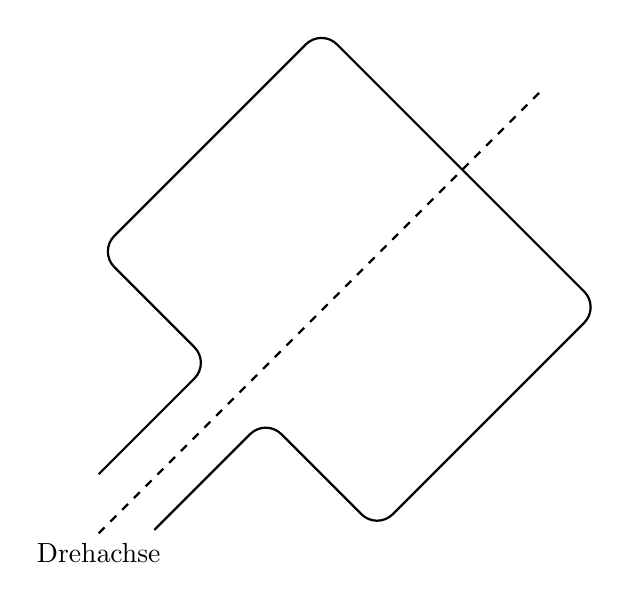
\begin{tikzpicture}
	\draw[thick,rounded corners=8pt] (0,0) -- ++(45:2) -- ++(135:2) -- ++(45:4) -- ++(-45:5) -- ++(-135:4) -- ++(135:2) -- ++(-135:2);
	\draw[thick, dashed] (0,-0.75) node[below] {Drehachse} -- +(45:8);
\end{tikzpicture}
\begin{lstlisting}[frame=single]
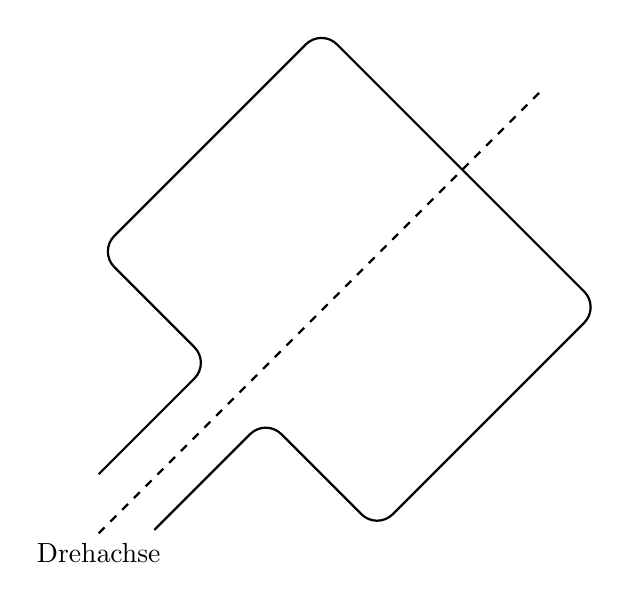
\begin{tikzpicture}
	\draw[thick,rounded corners=8pt] (0,0) -- ++(45:2) -- ++(135:2) -- ++(45:4) -- ++(-45:5) -- ++(-135:4) -- ++(135:2) -- ++(-135:2);
	\draw[thick, dashed] (0,-0.75) node[below] {Drehachse} -- +(45:8);
\end{tikzpicture}
\end{lstlisting}

\section{08.01.2009}
\subsection{08.01.2009-IMG-phys-1}
%Picture
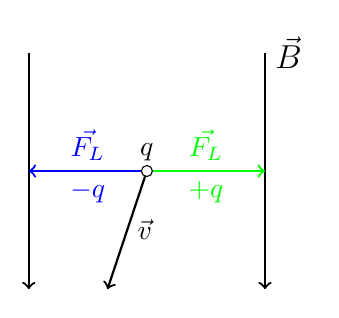
\begin{tikzpicture}
	\draw[->, thick] (0,0) -- (0,-3);
	\draw[->, thick] (3,0) node[right] {\large{$\vec{B}$}} -- (3,-3);

	\draw[->, thick, draw=green] (1.5,-1.5) -- (3,-1.5) node[above, midway, text=green] {$\vec{F_L}$} node[below, midway, text=green] {$+q$};
	\draw[->, thick, draw=blue] (1.5,-1.5) -- (0,-1.5) node[above, midway, text=blue] {$\vec{F_L}$} node[below, midway, text=blue] {$-q$};

	\draw[->, thick] (1.5,-1.5) -- (1,-3) node[right, midway] {$\vec{v}$};

	\draw[fill=white] (1.5,-1.5) circle (0.07) node[above] {$q$};
\end{tikzpicture}
%Code
\begin{lstlisting}[frame=single]
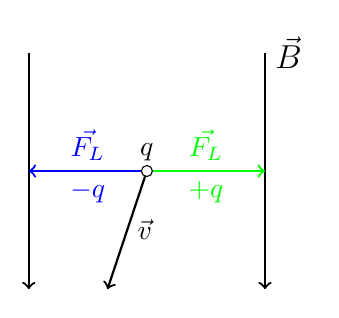
\begin{tikzpicture}
	\draw[->, thick] (0,0) -- (0,-3);
	\draw[->, thick] (3,0) node[right] {\large{$\vec{B}$}} -- (3,-3);

	\draw[->, thick, draw=green] (1.5,-1.5) -- (3,-1.5) node[above, midway, text=green] {$\vec{F_L}$} node[below, midway, text=green] {$+q$};
	\draw[->, thick, draw=blue] (1.5,-1.5) -- (0,-1.5) node[above, midway, text=blue] {$\vec{F_L}$} node[below, midway, text=blue] {$-q$};

	\draw[->, thick] (1.5,-1.5) -- (1,-3) node[right, midway] {$\vec{v}$};

	\draw[fill=white] (1.5,-1.5) circle (0.07) node[above] {$q$};
\end{tikzpicture}
\end{lstlisting}

\section{12.01.2009}
\subsection{12.01.2009-IMG-phys-1}
%Picture
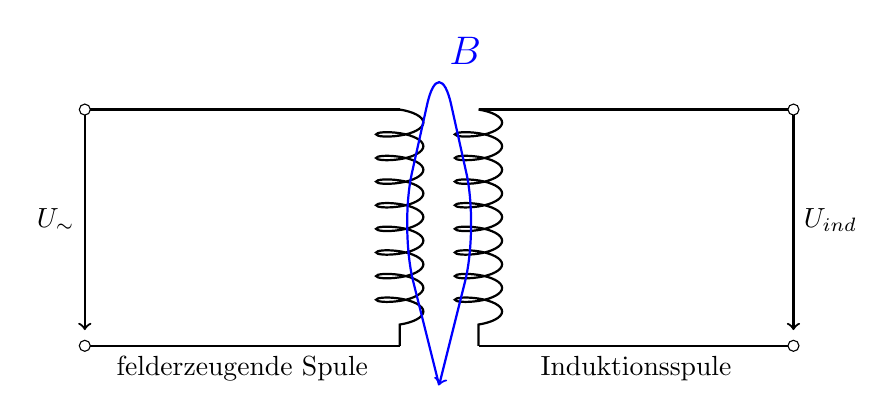
\begin{tikzpicture}[decoration={coil,aspect=0.3,segment length=3mm,amplitude=3mm}]

	%Linker Teil
	\draw[->, thick] (0,0) -- (0,-2.8) node[left, midway] {$U_{\sim}$};
	\draw[thick] (0,0) -- (4,0);
	\draw[thick] (4,-3) -- (0,-3) node[below, midway] {felderzeugende Spule};
	%Spule 1
	\draw[thick, decorate] (4,0) -- (4,-3);

	\draw[fill=white] (0,0) circle (0.07);
	\draw[fill=white] (0,-3) circle (0.07);

	%Rechter Teil
	\draw[thick] (5,0) -- (9,0);
	\draw[->, thick] (9,0) -- (9, -2.8) node[right, midway] {$U_{ind}$};
	\draw[thick] (5,-3) -- (9,-3) node[below, midway] {Induktionsspule};
	%Spule 2
	\draw[thick, decorate] (5,0) -- (5,-3);

	\draw[fill=white] (9,0) circle (0.07);
	\draw[fill=white] (9,-3) circle (0.07);

	\draw[thick, draw=blue, ->, rounded corners=20pt] (4.5,-3.5) -- (4,-1.5) -- (4.5,0.75) node[right, text=blue] {\Large{$B$}} -- (5,-1.5) -- (4.5,-3.5);
\end{tikzpicture}
%Code
\begin{lstlisting}[frame=single]
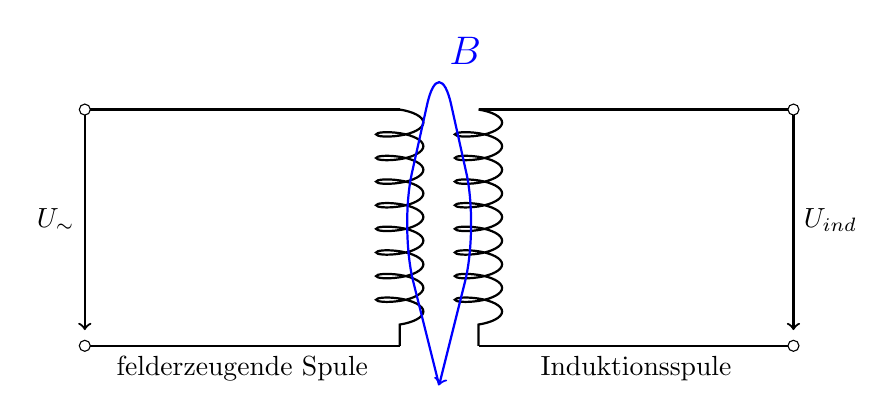
\begin{tikzpicture}[decoration={coil,aspect=0.3,segment length=3mm,amplitude=3mm}]

	%Linker Teil
	\draw[->, thick] (0,0) -- (0,-2.8) node[left, midway] {$U_{\sim}$};
	\draw[thick] (0,0) -- (4,0);
	\draw[thick] (4,-3) -- (0,-3) node[below, midway] {felderzeugende Spule};
	%Spule 1
	\draw[thick, decorate] (4,0) -- (4,-3);

	\draw[fill=white] (0,0) circle (0.07);
	\draw[fill=white] (0,-3) circle (0.07);

	%Rechter Teil
	\draw[thick] (5,0) -- (9,0);
	\draw[->, thick] (9,0) -- (9, -2.8) node[right, midway] {$U_{ind}$};
	\draw[thick] (5,-3) -- (9,-3) node[below, midway] {Induktionsspule};
	%Spule 2
	\draw[thick, decorate] (5,0) -- (5,-3);

	\draw[fill=white] (9,0) circle (0.07);
	\draw[fill=white] (9,-3) circle (0.07);

	\draw[thick, draw=blue, ->, rounded corners=20pt] (4.5,-3.5) -- (4,-1.5) -- (4.5,0.75) node[right, text=blue] {\Large{$B$}} -- (5,-1.5) -- (4.5,-3.5);
\end{tikzpicture}
\end{lstlisting}

\subsection{12.01.2009-IMG-phys-4}
%Picture
\begin{tikzpicture}
	\draw[->, thick] (0,0) node[left] {$B$} -- (0,3) node[left] {$U_N$};
	\draw[->, thick] (-0.2,1.5) node[left] {$I$} -- (5,1.5) node[below] {$t$};
	\draw (0,2.5) -- (5,2.5);
\end{tikzpicture}
%Code
\begin{lstlisting}[frame=single]
\begin{tikzpicture}
	\draw[->, thick] (0,0) node[left] {$B$} -- (0,3) node[left] {$U_N$};
	\draw[->, thick] (-0.2,1.5) node[left] {$I$} -- (5,1.5) node[below] {$t$};
	\draw (0,2.5) -- (5,2.5);
\end{tikzpicture}
\end{lstlisting}

\subsection{12.01.2009-IMG-phys-5}
%Picture
\begin{tikzpicture}
	\draw[->, thick] (0,0) -- (0,3);
	\draw[->, thick] (-0.2,1.5) node[left] {$0$} -- (5,1.5) node[below] {$t$} node[below, midway] {$U_{ind} > 0$};
\end{tikzpicture}
%Code
\begin{lstlisting}[frame=single]
\begin{tikzpicture}
	\draw[->, thick] (0,0) -- (0,3);
	\draw[->, thick] (-0.2,1.5) node[left] {$0$} -- (5,1.5) node[below] {$t$} node[below, midway] {$U_{ind} > 0$};
\end{tikzpicture}
\end{lstlisting}
\chapter{Mathematik}
\section{05.11.2008}
\subsection{05.11.2008-IMG-mathe-4}
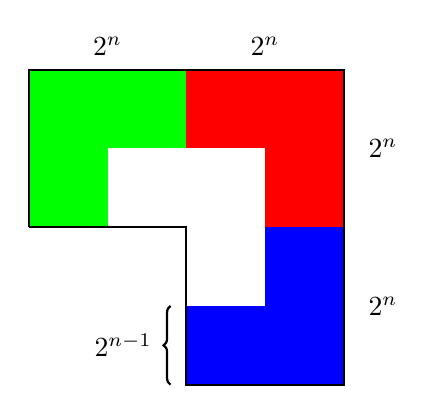
\begin{tikzpicture}[thick]
	\fill[fill=green] (0,0) rectangle (1,2);
	\fill[fill=green] (1,2) rectangle (2,1);

	\fill[fill=red] (2,2) rectangle (4,1);
	\fill[fill=red] (3,1) rectangle (4,0);

	\fill[fill=blue] (3,0) rectangle (4,-2);
	\fill[fill=blue] (3,-2) rectangle (2,-1);

	\draw (0,0) -- (2,0) -- (2,-2) -- (4,-2) -- (4,2) -- (0,2) -- (0,0);

	\node at (1,2.3) {$2^n$};
	\node at (3,2.3) {$2^n$};
	\node at (4.5,1) {$2^n$};
	\node at (4.5,-1) {$2^n$};
	\draw decorate [decoration=brace] {(1.8,-2) -- (1.8,-1)};
	\node at (1.2,-1.5) {$2^{n-1}$};
\end{tikzpicture}
\begin{lstlisting}[frame=single]
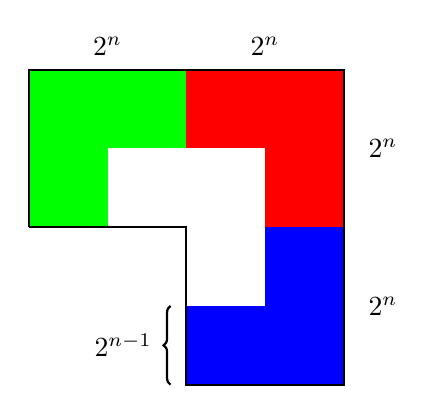
\begin{tikzpicture}[thick]
	\fill[fill=green] (0,0) rectangle (1,2);
	\fill[fill=green] (1,2) rectangle (2,1);

	\fill[fill=red] (2,2) rectangle (4,1);
	\fill[fill=red] (3,1) rectangle (4,0);

	\fill[fill=blue] (3,0) rectangle (4,-2);
	\fill[fill=blue] (3,-2) rectangle (2,-1);

	\draw (0,0) -- (2,0) -- (2,-2) -- (4,-2) -- (4,2) -- (0,2) -- (0,0);

	\node at (1,2.3) {$2^n$};
	\node at (3,2.3) {$2^n$};
	\node at (4.5,1) {$2^n$};
	\node at (4.5,-1) {$2^n$};
	\draw decorate [decoration=brace] {(1.8,-2) -- (1.8,-1)};
	\node at (1.2,-1.5) {$2^{n-1}$};
\end{tikzpicture}
\end{lstlisting}

\subsection{05.11.2008-IMG-mathe-5}
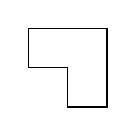
\begin{tikzpicture}
	\draw (0,0) -- (0,0.5) -- (1,0.5) -- (1,-0.5) -- (0.5,-0.5) -- (0.5,0) -- (0,0);
\end{tikzpicture}
\begin{lstlisting}[frame=single]
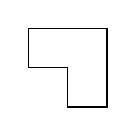
\begin{tikzpicture}
	\draw (0,0) -- (0,0.5) -- (1,0.5) -- (1,-0.5) -- (0.5,-0.5) -- (0.5,0) -- (0,0);
\end{tikzpicture}
\end{lstlisting}

\subsection{05.11.2008-IMG-mathe-6}
\begin{tikzpicture}
	\draw (0,0) rectangle (0.5,0.5);

	\node at (0.25,0.8) {$1$};
	\node at (0.8,0.25) {$1$};
\end{tikzpicture}
\begin{lstlisting}[frame=single]
\begin{tikzpicture}
	\draw (0,0) rectangle (0.5,0.5);

	\node at (0.25,0.8) {$1$};
	\node at (0.8,0.25) {$1$};
\end{tikzpicture}
\end{lstlisting}

\subsection{05.11.2008-IMG-mathe-7}
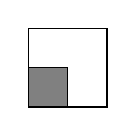
\begin{tikzpicture}
	\draw (0,0) rectangle (1,1);
	\draw[fill=gray] (0,0) rectangle (0.5,0.5);
\end{tikzpicture}
\begin{lstlisting}[frame=single]
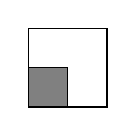
\begin{tikzpicture}
	\draw (0,0) rectangle (1,1);
	\draw[fill=gray] (0,0) rectangle (0.5,0.5);
\end{tikzpicture}
\end{lstlisting}

\subsection{05.11.2008-IMG-mathe-8}
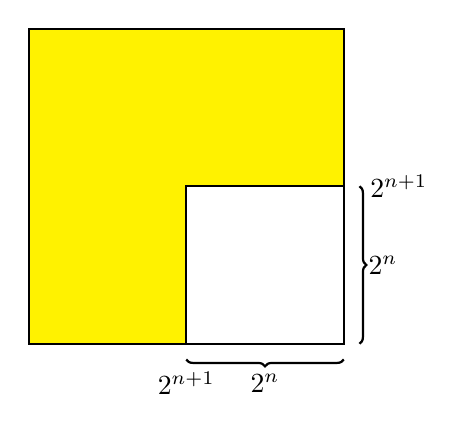
\begin{tikzpicture}[thick]
	\draw[fill=yellow] (0,0) rectangle (4,4);
	\draw[fill=white] (2,2) rectangle (4,0);

	\draw decorate [decoration=brace]  {(4,-0.2) -- (2,-0.2)};
	\draw decorate [decoration=brace] {(4.2,2) -- (4.2,0)};

	\node at (2,-0.5) {$2^{n+1}$};
	\node at (4.7,2) {$2^{n+1}$};
	\node at (3,-0.5) {$2^n$};
	\node at (4.5,1) {$2^n$};
\end{tikzpicture}
\begin{lstlisting}[frame=single]
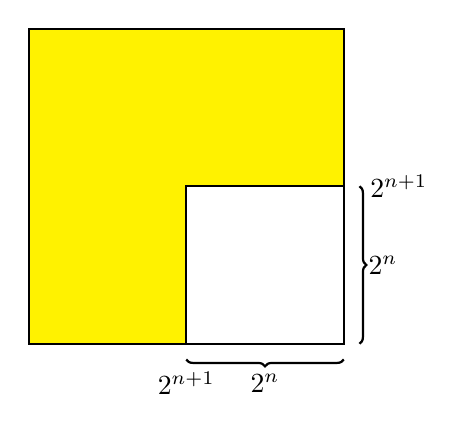
\begin{tikzpicture}[thick]
	\draw[fill=yellow] (0,0) rectangle (4,4);
	\draw[fill=white] (2,2) rectangle (4,0);

	\draw decorate [decoration=brace]  {(4,-0.2) -- (2,-0.2)};
	\draw decorate [decoration=brace] {(4.2,2) -- (4.2,0)};

	\node at (2,-0.5) {$2^{n+1}$};
	\node at (4.7,2) {$2^{n+1}$};
	\node at (3,-0.5) {$2^n$};
	\node at (4.5,1) {$2^n$};
\end{tikzpicture}
\end{lstlisting}

\subsection{05.11.2008-IMG-mathe-9}

\begin{tikzpicture}
	\fill[fill=yellow] (0,0) rectangle (0.5,1);
	\fill[fill=yellow] (0.5,1) rectangle (1,0.5);
	\draw (0,0) -- (0,1) -- (1,1) -- (1,0.5) -- (0.5,0.5) -- (0.5,0) -- (0,0);
\end{tikzpicture}
\begin{lstlisting}[frame=single]

\begin{tikzpicture}
	\fill[fill=yellow] (0,0) rectangle (0.5,1);
	\fill[fill=yellow] (0.5,1) rectangle (1,0.5);
	\draw (0,0) -- (0,1) -- (1,1) -- (1,0.5) -- (0.5,0.5) -- (0.5,0) -- (0,0);
\end{tikzpicture}
\end{lstlisting}

\subsection{05.11.2008-IMG-mathe-10}
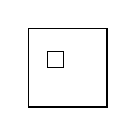
\begin{tikzpicture}
	\draw (0,0) rectangle (1,1);
	\draw (0.25,0.5) rectangle (0.45,0.7);
\end{tikzpicture}
\begin{lstlisting}[frame=single]
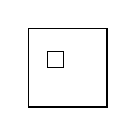
\begin{tikzpicture}
	\draw (0,0) rectangle (1,1);
	\draw (0.25,0.5) rectangle (0.45,0.7);
\end{tikzpicture}
\end{lstlisting}

\subsection{IMG-05.11.2008-mathe-3}
\begin{tikzpicture}
	\draw (0,0) -- (2,0) -- (2,-2) -- (4,-2) -- (4,2) -- (0,2) -- (0,0);

	\draw[dashed] (2,0) -- (2,2);
	\draw[dashed] (2,0) -- (4,0);

	\node at (1,2.3) {$2^{n-1}$};
	\node at (3,2.3) {$2^{n-1}$};
	\node at (4.5,1) {$2^{n-1}$};
	\node at (4.5,-1) {$2^{n-1}$};
\end{tikzpicture}
\begin{lstlisting}[frame=single]
\begin{tikzpicture}
	\draw (0,0) -- (2,0) -- (2,-2) -- (4,-2) -- (4,2) -- (0,2) -- (0,0);

	\draw[dashed] (2,0) -- (2,2);
	\draw[dashed] (2,0) -- (4,0);

	\node at (1,2.3) {$2^{n-1}$};
	\node at (3,2.3) {$2^{n-1}$};
	\node at (4.5,1) {$2^{n-1}$};
	\node at (4.5,-1) {$2^{n-1}$};
\end{tikzpicture}
\end{lstlisting}

\section{11.12.2008}
\subsection{11.12.2008-IMG-mathe-1}
\definecolor{lightergray}{HTML}{DDDDDD}
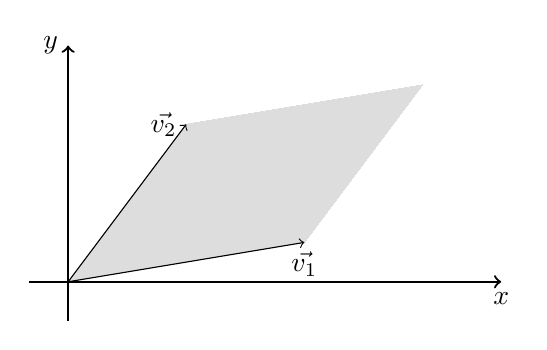
\begin{tikzpicture}
	\draw[fill=lightergray, line width=0pt, draw=lightergray] (0,0) -- (1.5,2) -- (4.5,2.5) -- (3,0.5) -- (0,0);

	\draw[->] (0,0) -- (1.5,2) node[left] {$\vec{v_2}$};
	\draw[->] (0,0) -- (3,0.5) node[below] {$\vec{v_1}$};

	\draw[->, thick] (-0.5,0) -- (5.5,0) node[below] {$x$};
	\draw[->, thick] (0,-0.5) -- (0,3) node[left] {$y$};
\end{tikzpicture}
\begin{lstlisting}[frame=single]
\definecolor{lightergray}{HTML}{DDDDDD}
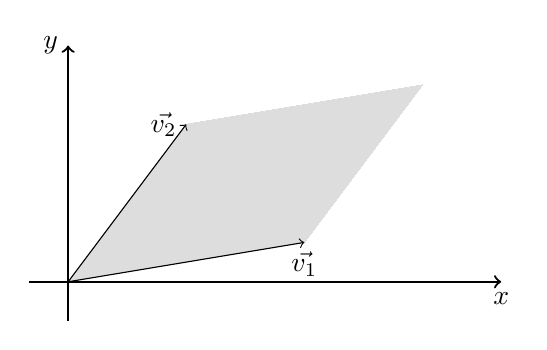
\begin{tikzpicture}
	\draw[fill=lightergray, line width=0pt, draw=lightergray] (0,0) -- (1.5,2) -- (4.5,2.5) -- (3,0.5) -- (0,0);

	\draw[->] (0,0) -- (1.5,2) node[left] {$\vec{v_2}$};
	\draw[->] (0,0) -- (3,0.5) node[below] {$\vec{v_1}$};

	\draw[->, thick] (-0.5,0) -- (5.5,0) node[below] {$x$};
	\draw[->, thick] (0,-0.5) -- (0,3) node[left] {$y$};
\end{tikzpicture}
\end{lstlisting}

\subsection{11.12.2008-IMG-mathe-2}
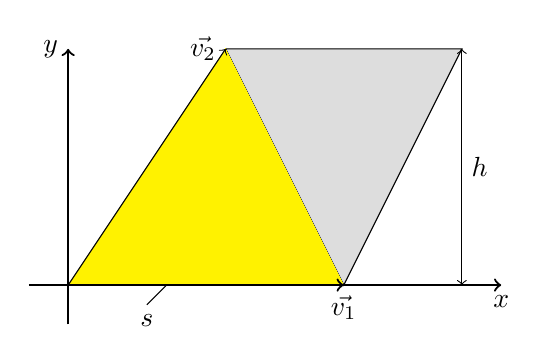
\begin{tikzpicture}
	\draw[fill=lightergray] (2,3) -- (3.5,0) -- (5,3) -- (2,3); 

	\draw[fill=yellow, line width=0pt, draw=yellow] (0,0) -- (2,3) -- (3.5,0) -- (0,0);

	\draw[->] (0,0) -- (2,3) node[left] {$\vec{v_2}$};
	\draw[->, thick] (0,0) -- (3.5,0) node[below] {$\vec{v_1}$};
	\draw (1.25,0) -- (1,-0.25) node[below] {$s$};
	\draw[<->] (5,3) -- (5,0);
	\node[right] at (5,1.5) {$h$};

	\draw[->, thick] (-0.5,0) -- (5.5,0) node[below] {$x$};
	\draw[->, thick] (0,-0.5) -- (0,3) node[left] {$y$};
\end{tikzpicture}
\begin{lstlisting}[frame=single]
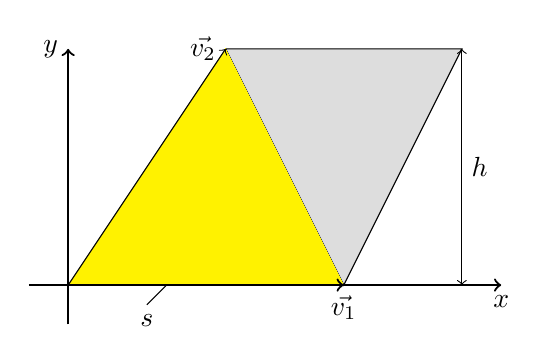
\begin{tikzpicture}
	\draw[fill=lightergray] (2,3) -- (3.5,0) -- (5,3) -- (2,3); 

	\draw[fill=yellow, line width=0pt, draw=yellow] (0,0) -- (2,3) -- (3.5,0) -- (0,0);

	\draw[->] (0,0) -- (2,3) node[left] {$\vec{v_2}$};
	\draw[->, thick] (0,0) -- (3.5,0) node[below] {$\vec{v_1}$};
	\draw (1.25,0) -- (1,-0.25) node[below] {$s$};
	\draw[<->] (5,3) -- (5,0);
	\node[right] at (5,1.5) {$h$};

	\draw[->, thick] (-0.5,0) -- (5.5,0) node[below] {$x$};
	\draw[->, thick] (0,-0.5) -- (0,3) node[left] {$y$};
\end{tikzpicture}
\end{lstlisting}

\subsection{11.12.2008-IMG-mathe-3}
\begin{tikzpicture}
	\draw[->, thick] (0,0) -- (6,0) node[right] {$y$};
	\draw[->, thick] (0,0) -- (0,7) node[left] {$z$};
	\draw[->, thick] (0,0) -- (-2,-2.5) node[below] {$x$};

	\draw[draw=gray, nearly opaque, thick] (-1,-2) -- (-1,4) -- (2,4) -- (2,-2) -- (-1,-2);
	\draw[draw=gray, nearly opaque, thick] (-1,4) -- (1,6) -- (4,6) -- (2,4);
	\draw[draw=gray, nearly opaque, thick] (2,-2) -- (4,0) -- (4,6) node [above] {\LARGE{$V$}};
\end{tikzpicture}
\begin{lstlisting}[frame=single]
\begin{tikzpicture}
	\draw[->, thick] (0,0) -- (6,0) node[right] {$y$};
	\draw[->, thick] (0,0) -- (0,7) node[left] {$z$};
	\draw[->, thick] (0,0) -- (-2,-2.5) node[below] {$x$};

	\draw[draw=gray, nearly opaque, thick] (-1,-2) -- (-1,4) -- (2,4) -- (2,-2) -- (-1,-2);
	\draw[draw=gray, nearly opaque, thick] (-1,4) -- (1,6) -- (4,6) -- (2,4);
	\draw[draw=gray, nearly opaque, thick] (2,-2) -- (4,0) -- (4,6) node [above] {\LARGE{$V$}};
\end{tikzpicture}
\end{lstlisting}

\section{08.01.2009}
\subsection{08.01.2009-IMG-math-1}
%Picture
\begin{tikzpicture}
	\node at (0,0) (Vl) {$V$};
	\node at (3,0) (Vr) {$V$};
	\node at (0,3) (Kl) {$K^n$};
	\node at (3,3) (Kr) {$K^n$};

	\draw[->] (Vl.north) -- (Kl.south);
	\draw[->] (Vl.east) -- (Vr.west) node[above, midway] {$f$};

	\draw[->] (Kl.east) -- (Kr.west) node[below, midway] {$f$};

	\draw[->] (Kr.south) -- (Vr.north);
\end{tikzpicture}
%Code
\begin{lstlisting}[frame=single]
\begin{tikzpicture}
	\node at (0,0) (Vl) {$V$};
	\node at (3,0) (Vr) {$V$};
	\node at (0,3) (Kl) {$K^n$};
	\node at (3,3) (Kr) {$K^n$};

	\draw[->] (Vl.north) -- (Kl.south);
	\draw[->] (Vl.east) -- (Vr.west) node[above, midway] {$f$};

	\draw[->] (Kl.east) -- (Kr.west) node[below, midway] {$f$};

	\draw[->] (Kr.south) -- (Vr.north);
\end{tikzpicture}
\end{lstlisting}

\section{14.01.2009}
\subsection{14.01.2009-IMG-mathe-1}
%Picture
\begin{tikzpicture}
	\draw[thick, <->] (3,0) -- (0,0) -- (0,3);

	\draw[->] (0,0) -- (2,2) node[left, midway] {$\vec{v}$};
	\draw[draw=blue, thick] (0,0) -- (2,0) node[below, midway, text=blue] {$U_1$};
	\draw[draw=blue] (2,0) -- (2,2) node[right, midway, text=blue] {$U_2$};
	\draw[draw=blue] (1.7,0) arc (180:90:0.3);
	\draw[draw=blue, fill=blue] (1.9,0.125) circle (0.02);
\end{tikzpicture}
%Code
\begin{lstlisting}[frame=single]
\begin{tikzpicture}
	\draw[thick, <->] (3,0) -- (0,0) -- (0,3);

	\draw[->] (0,0) -- (2,2) node[left, midway] {$\vec{v}$};
	\draw[draw=blue, thick] (0,0) -- (2,0) node[below, midway, text=blue] {$U_1$};
	\draw[draw=blue] (2,0) -- (2,2) node[right, midway, text=blue] {$U_2$};
	\draw[draw=blue] (1.7,0) arc (180:90:0.3);
	\draw[draw=blue, fill=blue] (1.9,0.125) circle (0.02);
\end{tikzpicture}
\end{lstlisting}

\subsection{14.01.2009-IMG-mathe-2}
%Picture
\begin{tikzpicture}
	\draw[->, thick] (0,0) -- (3,0) node[below, midway] {$\vec{u}$};
	\draw[->, thick] (0,0) -- (45:1.5) node[left, midway] {$\vec{r}$};
	\draw[thick] (0.8,0) arc (0:45:0.8);
	\path (0,0) ++(22.5:0.5) node{$\alpha$};
\end{tikzpicture}
%Code
\begin{lstlisting}[frame=single]
\begin{tikzpicture}
	\draw[->, thick] (0,0) -- (3,0) node[below, midway] {$\vec{u}$};
	\draw[->, thick] (0,0) -- (45:1.5) node[left, midway] {$\vec{r}$};
	\draw[thick] (0.8,0) arc (0:45:0.8);
	\path (0,0) ++(22.5:0.5) node{$\alpha$};
\end{tikzpicture}
\end{lstlisting}

\subsection{14.01.2009-IMG-mathe-3}
%Picture
\begin{tikzpicture}
	\draw[->, thick] (0,0) -- (3,0) node[below, midway] {$\vec{u}$};
	\draw[->, thick] (0,0) -- (45:1.5) node[left, midway] {$\vec{v}$};
	\draw[thick] (0.8,0) arc (0:45:0.8);
	\path (0,0) ++(22.5:0.5) node{$\alpha$};
\end{tikzpicture}
%Code
\begin{lstlisting}[frame=single]
\begin{tikzpicture}
	\draw[->, thick] (0,0) -- (3,0) node[below, midway] {$\vec{u}$};
	\draw[->, thick] (0,0) -- (45:1.5) node[left, midway] {$\vec{v}$};
	\draw[thick] (0.8,0) arc (0:45:0.8);
	\path (0,0) ++(22.5:0.5) node{$\alpha$};
\end{tikzpicture}
\end{lstlisting}

\subsection{14.01.2009-IMG-mathe-4}
%Picture
\begin{tikzpicture}
	\draw[->, thick] (-1.5,0) -- (1.5,0) node[below] {$x$};
	\draw[->, thick] (0,-0.5) -- (0,1);
	\draw[smooth] plot[domain=-3:3, scale=0.5] (\x,{cos(\x r)});
\end{tikzpicture}
%Code
\begin{lstlisting}[frame=single]
\begin{tikzpicture}
	\draw[->, thick] (-1.5,0) -- (1.5,0) node[below] {$x$};
	\draw[->, thick] (0,-0.5) -- (0,1);
	\draw[smooth] plot[domain=-3:3, scale=0.5] (\x,{cos(\x r)});
\end{tikzpicture}
\end{lstlisting}

\section{15.01.2009}
\subsection{15.01.2009-IMG-mathe-1}
%Picture
\begin{tikzpicture}
	\draw[<->, thick] (0,3) -- (0,0) node[left, midway] {$\vec{v}$} -- (5,0) node[below, midway] {$\vec{u}$};
	\draw[thick] (0,0.5) arc (90:0:0.5);
	\path (0,0) ++(45:0.25) node{$\alpha$};
\end{tikzpicture}
%Code
\begin{lstlisting}[frame=single]
\begin{tikzpicture}
	\draw[<->, thick] (0,3) -- (0,0) node[left, midway] {$\vec{v}$} -- (5,0) node[below, midway] {$\vec{u}$};
	\draw[thick] (0,0.5) arc (90:0:0.5);
	\path (0,0) ++(45:0.25) node{$\alpha$};
\end{tikzpicture}
\end{lstlisting}

\subsection{15.01.2009-IMG-mathe-2}
%Picture
\begin{tikzpicture}
	\draw[->, thick] (0,0) -- (3,3) node[left, midway] {$\vec{u} + \vec{v}$};
	\draw[->, thick] (0,0) -- (3,0) node[below, midway] {$\vec{u}$};
	\draw[->, thick] (3,0) -- (3,3) node[right, midway] {$\vec{v}$};
\end{tikzpicture}
%Code
\begin{lstlisting}[frame=single]
\begin{tikzpicture}
	\draw[->, thick] (0,0) -- (3,3) node[left, midway] {$\vec{u} + \vec{v}$};
	\draw[->, thick] (0,0) -- (3,0) node[below, midway] {$\vec{u}$};
	\draw[->, thick] (3,0) -- (3,3) node[right, midway] {$\vec{v}$};
\end{tikzpicture}
\end{lstlisting}

\subsection{15.01.2009-IMG-mathe-3}
%Picture
\begin{tikzpicture}
	\draw[thick] (0,0) -- (45:4);
	\draw[thick] (45:2) -- +(135:1);
	\draw[fill=black] (45:2) ++ (135:1) circle (0.04) node[left] {$A$};
	\draw[thick] (45:2) ++ (135:0.5) arc (135:45:0.5);
	\draw[fill=black] (45:2) ++ (90:0.25) circle (0.04);
\end{tikzpicture}
%Code
\begin{lstlisting}[frame=single]
\begin{tikzpicture}
	\draw[thick] (0,0) -- (45:4);
	\draw[thick] (45:2) -- +(135:1);
	\draw[fill=black] (45:2) ++ (135:1) circle (0.04) node[left] {$A$};
	\draw[thick] (45:2) ++ (135:0.5) arc (135:45:0.5);
	\draw[fill=black] (45:2) ++ (90:0.25) circle (0.04);
\end{tikzpicture}
\end{lstlisting}
